
\section{Graph Construction methodology }\label{sec:chem}

Thus far we have only applied a qualitative analysis on the relationships between species in a mechanism. Although this can educate us about the chemistry within a specific system, often a quantitative value for the rate of reaction between different species is required when undergoing scientific evaluation or policy advice. To obtain such results a chemical mechanism is placed within an atmospheric model, initial concentrations are supplied and the chemistry is propagated forwards\footnote{Or backwards if the adjoint is used. (see section PAGERANK APPLICATIONS)} in time. Currently, there exist three main model diagnostics which we may use to analyse the importance or role of a species from a simulation (model) output. 


\subsubsection{Concentration time series}

The simplest of these methods look at the abundance of a  species at a specific point in the atmosphere - its concentration. As time moves forwards, chemicals within the atmosphere undergo a range of reactions which result in the making and breaking of bonds - thus the changing from one species to another. 

Using the species concentration as a metric, we can map how it changes over time, and how in changing the initial concentrations of a simulation can produce different results. This can be useful for looking at a range of possible scenarios and evaluating the potential outcome after a pre-determined amount of time. An example would be through the use of policy-based simulations to predict changes in ...

Using a simple example from a Methane only subset of the MCM (\autoref{fig:concentration}), it is possible to observe the inverse relationship between \ch{NO2} and \ch{NO} using only their concentration profiles. Here nitrogen monoxide reacts with a \ch{Ro2} species to produce an RO and nitrogen dioxide.
This then photolyses back to nitrogen oxide, releasing oxygen which may go on to form ozone (REF NOX CYCLE IN INTRO). The latter part of this reaction is dependant on photons and therefore can only occur during daytime (mostly).
 
\begin{figure}[H]
     \centering
         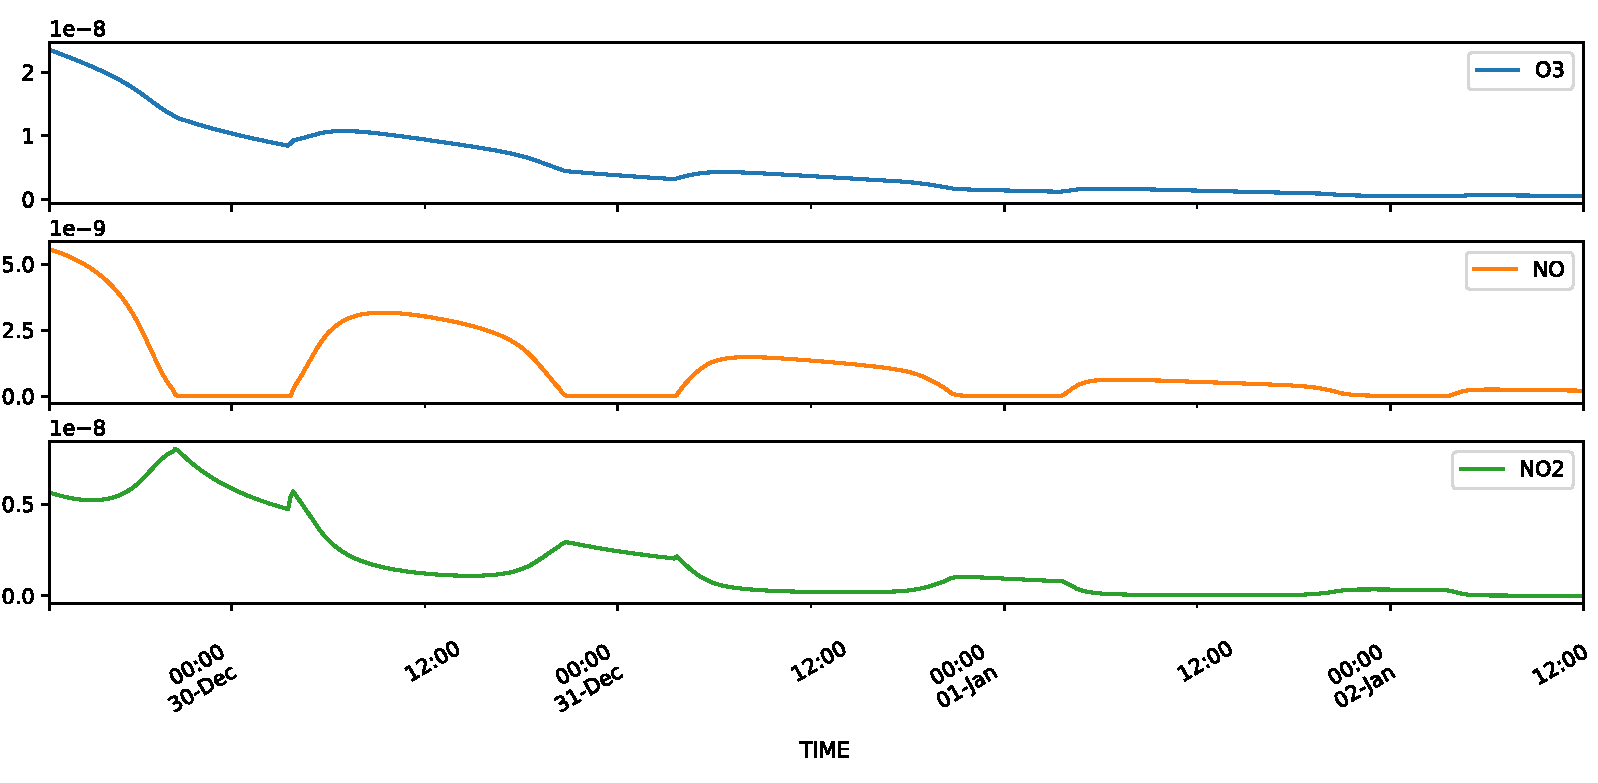
\includegraphics[width=.85\textwidth]{figures/ch2concentration.pdf}\\
         \ce{NO <-->[RO2][$hv$] NO2}.
        \caption{\textbf{A concentration time series from a simple methane-only simulation.} This is the simplest method for identifying changes in species within a model simulation. This multi-plot shows the changes in concentration profiles for all initialised species (NOx:10ppb; \ce{CH4}:20ppb; \ce{O3}:30ppb) following an initial 3 day spin-up to steady state. }
        \label{fig:concentration}
\end{figure}

\subsubsection{Rate of Production and Loss}

Analysing the concentration-time profiles allows the comparison of how a series of scenarios or runs change concerning their initial conditions and simulation length. Although these can tell us how, and how much, each species changes over time it does not rank or quantifies the specific reactions to which this may be attributed. Rate of Production Analysis (ROPA)\footnote{and loss} provides a method for establishing the total contribution from each reaction by calculating the change of concentration (concerning time) for the produced species - the instantaneous reaction Flux.

\begin{eqnarray}
  r_1 = \eta A + \omega B \overset{\kappa_1}{\xrightarrow{\hspace*{7mm}}} C & & \text{ Reaction 1}\\[15pt]
  f(C) = \dfrac{\delta C}{\delta t} =  [A][B]\  \eta \omega \times \kappa_1                      & & \text{ Instantanious Flux }(\Gamma) \label{eqn:ode}
\end{eqnarray}

Here A, B and C are example species; [A],[B] and [C] are species concentrations; $\eta$ and $\omega$ are rate coefficients and $\kappa$ is the rate of the reaction.  

Using a sample simulation representative of the conditions within Beijing (an urban environment), we explore the reactions contributing to the production and loss of \ch{CH3CO3},
\autoref{fig:ropa_day} at noon. The main reason for this specific example is that it can demonstrate how isolating a specific cause for the change within a species concentration may prove difficult in the context of atmospheric chemistry. Here we have many similarly weighted production and loss reaction, including that of peroxyacetyl nitrate (PAN) and nitrogen dioxide: 
\ce{CH3CO3 + NO2 <--> CH3C(O)ONO2} (PAN). The reversible nature, coupled with its near-identical production and loss fluxes produce a very small net change within our species of interest (\ch{CH3CO3}). Although this may be seen by calculating the cumulative flux between individual species, it is evident that simply looking at the concentrations or highest-ranking reaction fluxes may not be the best method of determining influence. To account for this we can look at how a change in one species can affect another using the Jacobian method.


\begin{figure}[H]
     \centering
         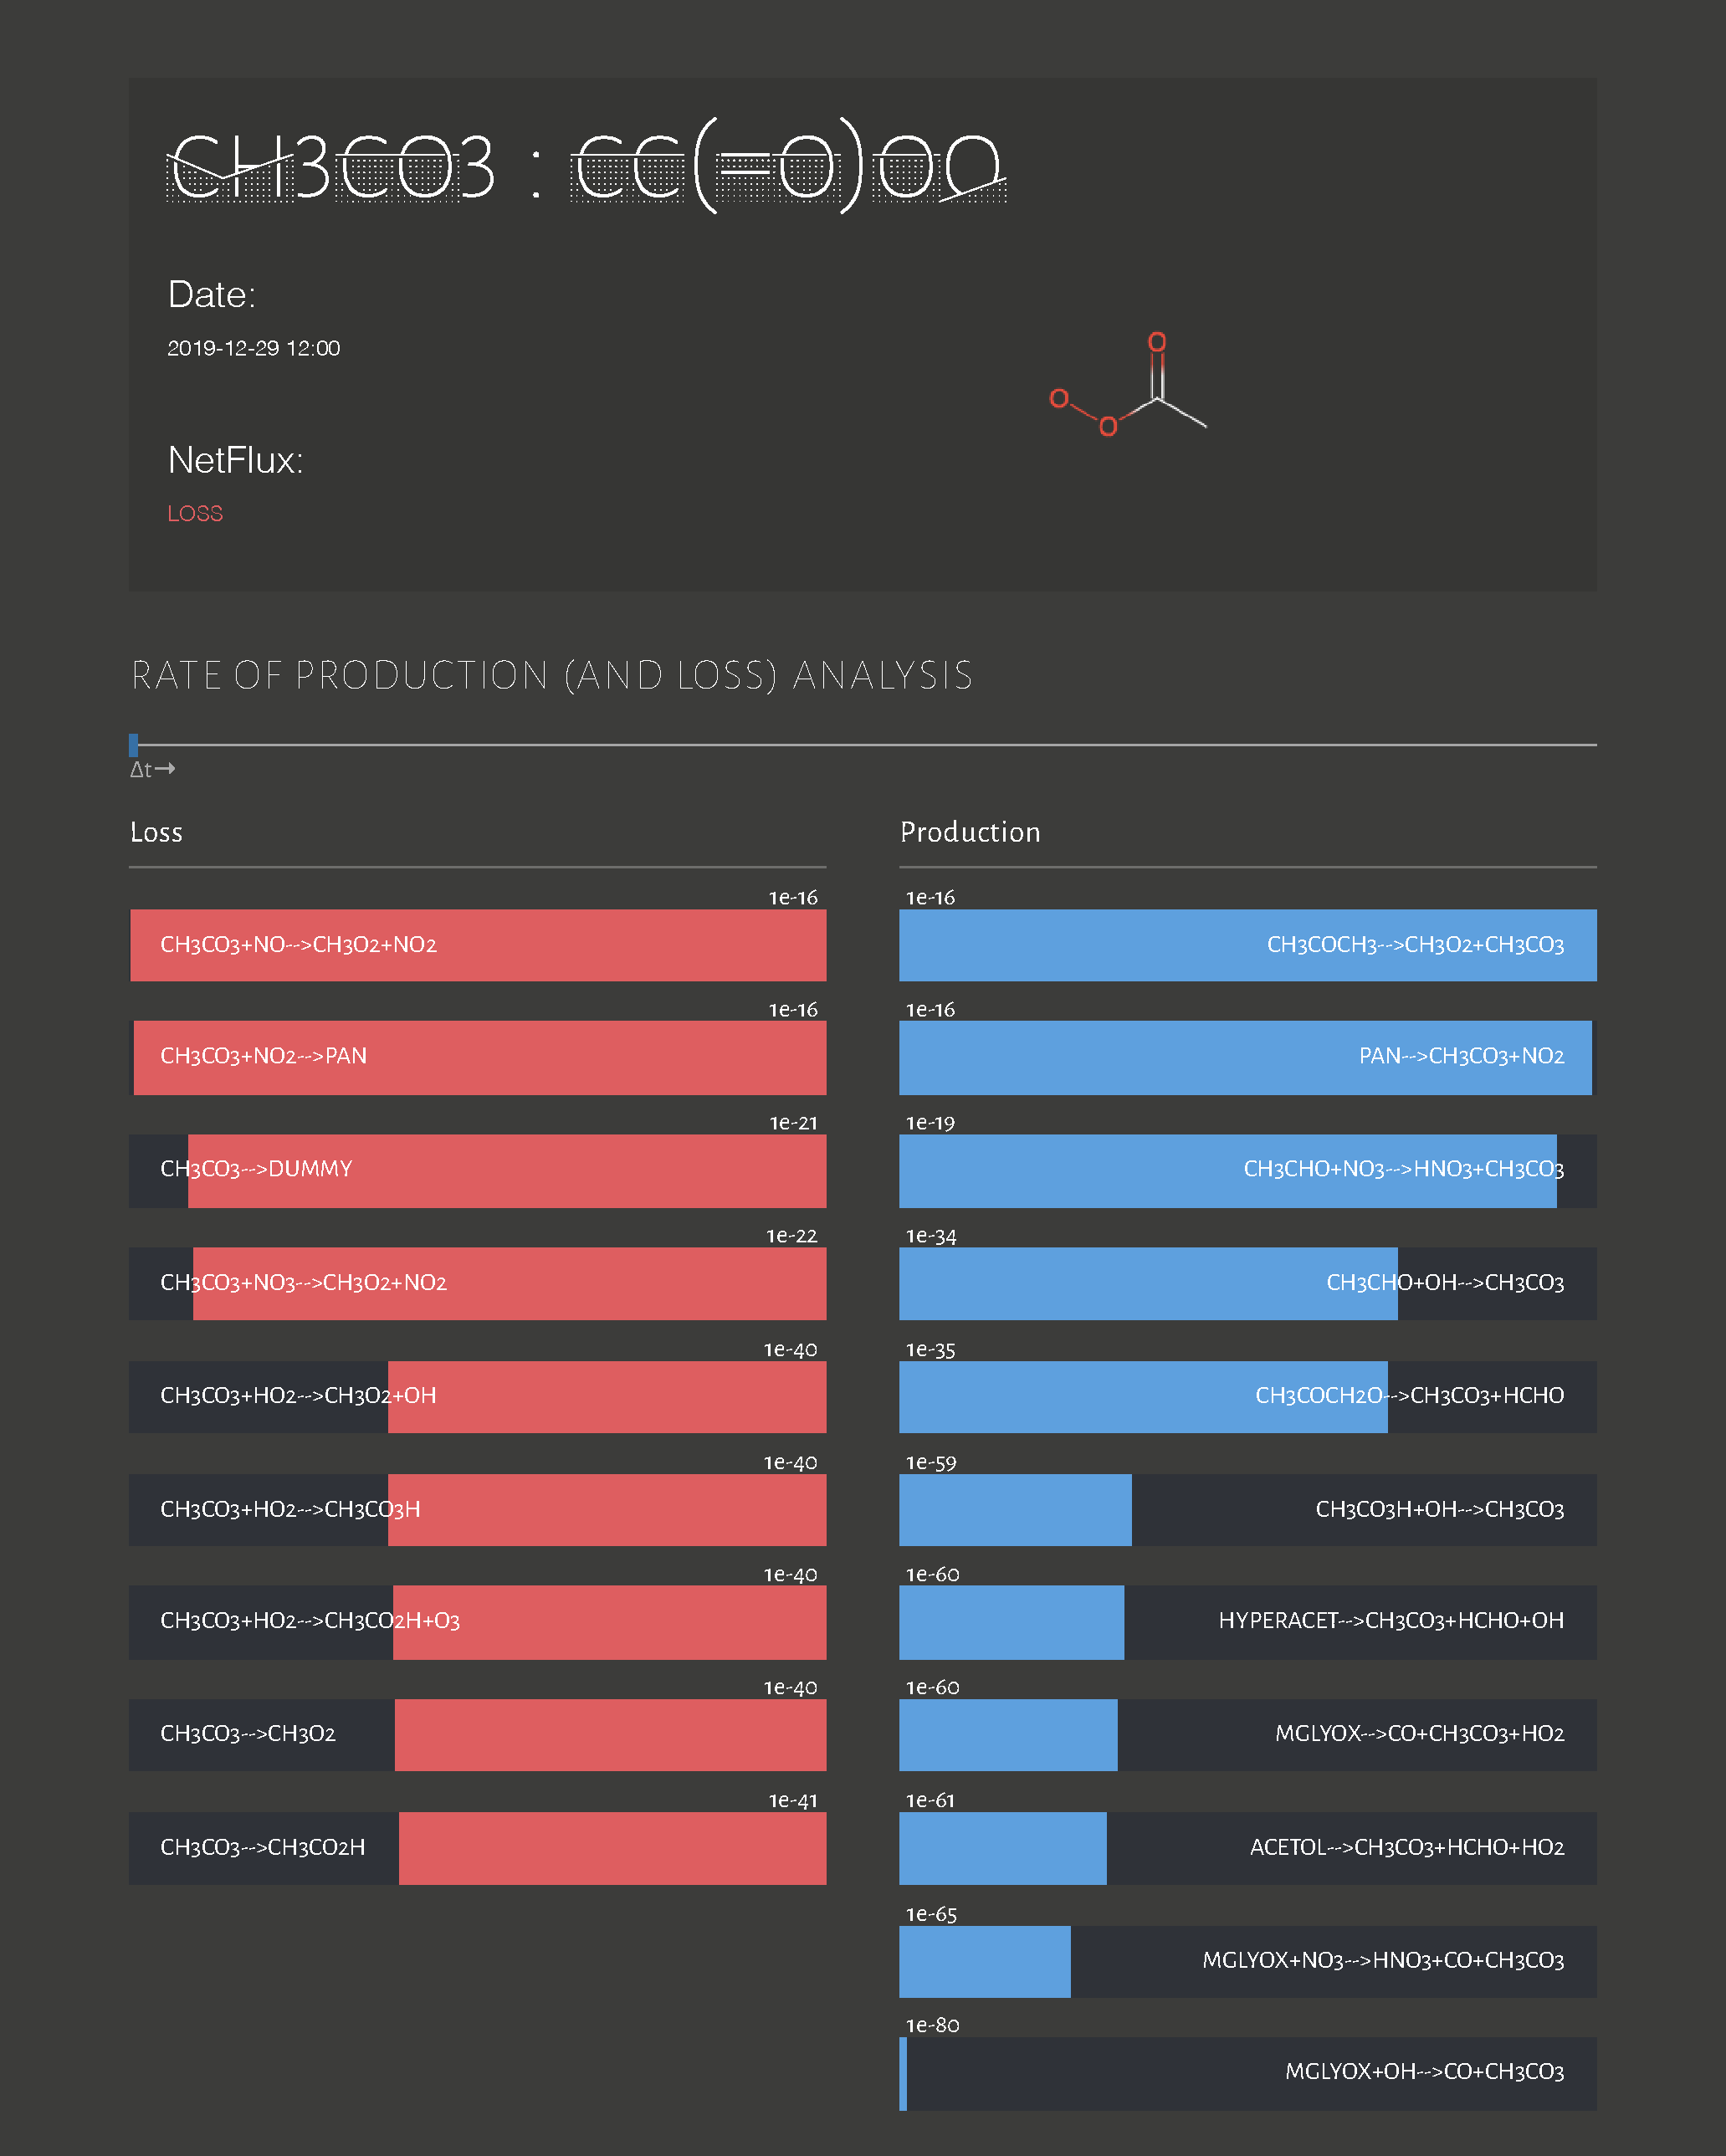
\includegraphics[width=\textwidth]{figures/ROPA_CH3CO3.pdf}
        \caption{\textbf{Rate of production and loss analysis plot for \ch{ch3co3} exhibiting a net loss (daytime).} An example ROPA plot from a simulation representing the chemistry within Beijing. This is used to identify the usefulness and weaknesses of using such a method.}
        \label{fig:ropa_day}
\end{figure}
\newpage



\subsubsection{The Jacobian}
"The Jacobian [matrix] generalises the notion of gradient to describe the sensitivity to a vector" - \cite{jacob}. That this means is that in taking the partial derivatives of each reaction flux (e.g. from \autoref{eqn:ode}), we can construct a representation of the influence each species has on itself - for example, the influence of species A on C and B on C (\autoref{eqn:A}-\ref{eqn:B}). 
\begin{eqnarray}
   \dfrac{\partial \ }{\partial A}\cdot \dfrac{\partial C_{r_1}}{\partial t} = \eta \omega B \kappa_1 & & \Gamma \text{ influence from A }\label{eqn:A}%\\[15pt]
\end{eqnarray}
    
\begin{eqnarray} 
   \dfrac{\partial \ }{\partial B}\cdot \dfrac{\partial C_{r_1}}{\partial t} = \eta \omega A \kappa_1 & &  \Gamma \text{ influence from B }\label{eqn:B}%\\[15pt]
\end{eqnarray}
      
These partial equations can then be aggregated for all reactions that contain the two species - taking the effect of species B on species C, for example, produces \autoref{eqn:Bsum}. Using these aggregate sums it is now possible to construct a pairwise relational matrix describing the influence each species has on every other species- \autoref{eqn:jacadj}. This is known as the jacobian matrix and is what is used to propagate the chemistry within a simulation forwards in time. 
 
               
\begin{eqnarray}
   \mathbf{J}_{C,B} = \dfrac{\partial f(C) }{\partial B} =
\dfrac{\partial \ }{\partial B} \cdot \left( \dfrac{\partial \Sigma_{r_1}}{\partial t} + \dfrac{\partial \Sigma_{r_2}}{\partial t} + \cdots +\dfrac{\partial \Sigma_{r_n}}{\partial t} \right)
\label{eqn:Bsum}
\end{eqnarray}\\

\begin{eqnarray}
 \mathbf{J}_{i,j} =
 \begin{bmatrix}
   \dfrac{\partial f_1}{\partial v_1} &
     \dfrac{\partial f_1}{\partial v_2} &
     \cdots &
     \dfrac{\partial f_1}{\partial v_n} \\[13pt]
   \dfrac{\partial f_2}{\partial v_1} &
     \dfrac{\partial f_2}{\partial v_2} &
       \cdots &
     \dfrac{\partial f_2}{\partial v_n} \\[13pt]
       \vdots &
     \vdots & \ddots
        &
     \vdots\\[13pt]
   \dfrac{\partial f_n}{\partial v_1} &
     \dfrac{\partial f_n}{\partial v_2} &
       \cdots &
     \dfrac{\partial f_n}{\partial v_n}
 \end{bmatrix}_{i,j=1}^{n,n}
 \label{eqn:jacadj}
\end{eqnarray}



\subsection{Graph construction methodology for simulated data}\label{sec:graphconstruction}

Having covered the general definition of a Jacobian matrix and how it is constructed, we can now apply it to the context of mechanism analysis and comprehension. The first analogy that needs to be made is that for the flux, we have a the first differential of a specific reaction in time. If we consider the change in a species concentration as a `displacement', we can think of the flux as its `velocity'.
Similarly, the Jacobian provides us with a description of how the individual flux of a species changes concerning the concentration (or displacement) or another species (the second-order partial differential). This is analogous to the acceleration of the object or particle we first displaced. In using the jacobian, we have constructed a relational matrix which outlines the effect a 1\% change of a species has on all other species - a concept which is the foundation of the connectivity method (a mechanism reduction technique where all but essential and important species are removed), \citep{connectivity}.

Since the format of a jacobian is already in the form of a relational matrix, it can easily be converted to a weighted adjacency matrix, and then directly into the graph format. Since it only considers the aggregated influence between species, much of the work that would otherwise be needed to convert a mechanism into a graph format has already been done. To make use of the Jacobian matrix, several extraction algorithms were written for an updated version of the Dynamically Simple Model of Atmospheric Chemical Complexity (DSMACC) [DANDSMACC,DSMACC ref], as discussed in INTRODUCTION. Here we edit the kinetic pre-processor output, \citep{kpp} to release the values of the Jacobian Matrix and return them at each model timestep for analysis. The process for how this is done is described in \autoref{sec:jacpractical}.



\subsubsection*{ A note on using the Flux instead of the Jacobian }
Depending on the model setup or the users' capabilities, extraction of the jacobian matrix for each timestep may not be possible. In many cases, the reaction rates and concentration may still be available, allowing for the calculation of reaction fluxes throughout the simulation. If this is the case the total flux can be calculated using the method described in  \autoref{eqn:ode}. From this, an edge-weighted by a reaction flux can be created from every reactant to each product. This generates a multi-graph\footnote{A graph with multiple edges between nodes} which may be simplified by taking the net flux value for all edges between two nodes. 

However, the potential for human/coding error, additional simplification and a non-explicit definition of the contribution of each species make the use of a Jacobian much more efficient in network generation from a chemical mechanism. 


\subsection{A practical Example using the MCM}\label{sec:jacpractical}

Taking a single equation from the MCM we may calculate the jacobian relationships between species and convert them into a graph. A randomly chosen ethane reaction (\autoref{eqn:line}) from a simple mechanism was chosen. It must be noted that in general it is unusual in the MCM that alkyl radicals react rapidly and extremely well with \ce{O2} to from stabilised peroxy radicals, \citep{mcmorigin}. In general, the reaction would consist of the following two steps:
 \ce{C2H6 + OH ->[\kappa_1] C2H5. + H2O}
and \ce{C2H5. + O2 -> [\kappa_2] CH2H5O2}.

\begin{equation}
\label{eqn:line}
\ce{C2H6} + \ce{OH} \overset{\kappa_3}{\xrightarrow{\hspace*{7mm}}} \ce{C2H5O2}
\end{equation}

For simplicity in this example, this will be the only equation for our mechanism. The resultant Flux \autoref{eqn:exflux} and resultant Jacobian \autoref{eqn:exjac} may be calculated.

\begin{equation}\label{eqn:exflux}
   \Gamma = [\ce{C2H6}][\ce{OH}]\kappa_1 \\[15pt]
\end{equation}

   \begin{eqnarray}
    \mathbf{J}_{i,j} =
 \begin{bmatrix}
   \dfrac{\partial f_{[\ce{C2H6}]}}{\partial t \ \partial {[\ce{C2H6}]}} &
     \dfrac{\partial f_{[\ce{C2H6}]}}{\partial {[\ce{OH}]}} &
     \dfrac{\partial f_{[\ce{C2H6}]}}{ t \partial {[\ce{C2H5O2}]}} \\[20pt]
   \dfrac{\partial f_{[\ce{OH}]}}{\partial t \ \partial {[\ce{C2H6}]}} &
     \dfrac{\partial f_{[\ce{OH}]}}{\partial t \ \partial {[\ce{OH}]}} &
   \dfrac{\partial f_{[\ce{OH}]}}{\partial t \ \partial {[\ce{C2H5O2}]}} \\[20pt]
   \dfrac{\partial f_{[\ce{C2H5O2}]}}{\partial t \ \partial {[\ce{C2H6}]}} &
     \dfrac{\partial f_{[\ce{C2H5O2}]}}{\partial t \ \partial {[\ce{OH}]}} &
     \dfrac{\partial f_{[\ce{C2H5O2}]}}{\partial t \ \partial {[\ce{C2H5O2}]}}
 \end{bmatrix}_{i,j=1}^{3,3}
 \label{eqn:exjac}
\end{eqnarray}\\


Since not all species react with all other species, we can remove reactions that do not exist. This forms a `sparse' jacobian. Substituting numbers from a subset mechanisms containing the methane and ethane precursors, we get \autoref{eqn:exjacsp}.


   \begin{eqnarray}
    \mathbf{J}_{i,j} =
 \begin{bmatrix}
   \dfrac{\partial f_{[\ce{C2H6}]}}{\partial t \ \partial {[\ce{C2H6}]}} &
     - 2\times 10^{-7} &
     2\times 10^{-7} \\[20pt]
   -0.1 &
     \dfrac{\partial f_{[\ce{OH}]}}{\partial t \ \partial {[\ce{OH}]}} &
  0.1 \\[20pt]
   \  &
    \  &
     \dfrac{\partial f_{[\ce{C2H5O2}]}}{\partial t \ \partial {[\ce{C2H5O2}]}}
 \end{bmatrix}_{i,j=1}^{3,3}
 \label{eqn:exjacsp}
\end{eqnarray}\\


This allows us to see two things. Firstly that with the absence of external intervention (e.g. emissions) the overall change of concentration is a conserved property. Secondly ...\\

Representing these relationships as a simple `ball and link' style graph gives us \autoref{fig:jacgraph}.

 \begin{figure}[H]
 \begin{center}
 \begin{tikzpicture}[->,>=stealth',shorten >=1pt,auto,node distance=7cm,
                    thick,main node/.style={circle,draw,font=\sffamily\small\bfseries}]

  \node[main node] (1) at (1,4){\ce{OH}};
  \node[main node] (2) at (1,0) {\ce{C2H6}};
  \node[main node] (3) at (7,2) {\ce{C2H5O2}};

  \path[every node/.style={font=\sffamily\small}]
    (1) edge [bend left] node {$2 \times 10^{-7}$} (3)
     (2) edge [bend right] node {$0.1$} (3);

     \path[every node/.style={font=\sffamily\small,color=orange}]
     (1) edge [bend left] node {$-2\times 10^{-7}$} (2)
     (2) edge [bend left] node {$-0.1$} (1);

        %edge [loop left] node {0.4} (2)
        %edge [bend right] node[left] {0.1} (3);
    %(3) edge node [right] {0.8} (2);
\end{tikzpicture}

 \end{center}

\caption{ A graphical representation of \autoref{eqn:exjacsp} derrived from the \autoref{eqn:line}}\label{fig:jacgraph}
 \end{figure}

\paragraph{Converting the Jacobian into an adjacency matrix}
Adjacency matrixes are a set of matrix representations which can be used in the construction of a graph. The relational data of the Jacobian matrix \autoref{eqn:exjacsp} inherently holds such property and can be directly translated to produce a graph, \autoref{fig:jacgraph}. However, we notice that some edge weights are negative, which although providing information about the chemical system provides no physical meaning in the graph structure.

It is for this reason that we can reverse the direction for all negative links to produce \autoref{fig:jacgraphnonneg}.

\begin{figure}[H]
\begin{center}
\begin{tikzpicture}[->,>=stealth',shorten >=1pt,auto,node distance=7cm,
                   thick,main node/.style={circle,draw,font=\sffamily\small\bfseries}]

 \node[main node] (1) at (1,4){\ce{OH}};
 \node[main node] (2) at (1,0) {\ce{C2H6}};
 \node[main node] (3) at (7,2) {\ce{C2H5O2}};

 \path[every node/.style={font=\sffamily\small,color=blue}]
   (1) edge [bend left] node {$2 \times 10^{-7}$} (3)
   (2) edge [bend left ] node {$2\times 10^{-7}$} (1);
   \path[every node/.style={font=\sffamily\small,color=red}]
   (1) edge [bend left] node {$0.1$} (2)
  (2) edge [bend right] node {$0.1$} (3);
\end{tikzpicture}

\end{center}

\caption{ Reversing the directions on negatively weighted edges from \autoref{fig:jacgraph}}\label{fig:jacgraphnonneg}
\end{figure}


For most graph algorithms this should be sufficient and is generally all that is needed. In some cases, it may, however, be noted that the graph may further be simplified to produce \autoref{fig:jacgraphsim}. Although this is more practical, eigenvector metrics such as PageRank will automatically transfer the `flow' of information down the system producing much the same overall result.

\begin{figure}[H]
\begin{center}
\begin{tikzpicture}[->,>=stealth',shorten >=1pt,auto,node distance=7cm,
                   thick,main node/.style={circle,draw,font=\sffamily\small\bfseries}]

 \node[main node] (1) at (1,4){\ce{OH}};
 \node[main node] (2) at (1,0) {\ce{C2H6}};
 \node[main node] (3) at (7,2) {\ce{C2H5O2}};

 \path[every node/.style={font=\sffamily\small,color=blue}]
   (2) edge [bend right] node {$2 \times 10^{-7}$} (3);
   \path[every node/.style={font=\sffamily\small,color=red}]
  (1) edge [bend left] node {$0.1$} (3);
\end{tikzpicture}

\end{center}

\caption{ Simplifying \autoref{fig:jacgraphnonneg}}
\label{fig:jacgraphsim}
\end{figure}
